%================================================================
\section{Results and Discussion}\label{sec:Results}
%================================================================

The programs containing the implementation of the methods discussed in the previous section, as well as the results presented in this section, can be found at the GitHub repository
\begin{center}
    \url{https://github.com/nicolossus/FYS-STK4155-Project2}
\end{center}

The procedures for producing the following results are contained in Jupyter Notebooks found \href{https://github.com/nicolossus/FYS-STK4155-Project2/tree/master/notebooks}{here}.


%----------------------------------------------------------------
\subsection{Producing Data for 1D Ising Model}\label{sec:results datagen}
%----------------------------------------------------------------

Discuss counting in the all-to-all Ising model

When doing the regression we included both $s_js_i$ and $s_is_j$ for all $i,j$ in the features. Since these quantities are equal, we do not get a unique solution for OLS, so we resort to SVD. SVD gives the coefficients with the least $L2$-norm. Hence we tend to get solutions $J_{i,j}=J_{j,i}=-0.5$. Ridge is similar in this regard, since it uses an $L2$ penalty. Lasso uses the $L1$-norm which doesn't differentiate between e.g. $J_{i,j}=-1$ and $J_{j,i} = 0$ on one hand and $J_{i,j}=J_{j,i}=-0.5$ on the other. Lasso tends to give coefficients which are equal to zero, which is consistent with what we have observed here.

%----------------------------------------------------------------
\subsection{Learning the Ising Hamiltonian with Linear Regression}\label{sec:results linreg}
%----------------------------------------------------------------

\autoref{fig:j_ols} shows the coupling matrix obtained by performing OLS regression.

\begin{figure}[H]
\begin{center}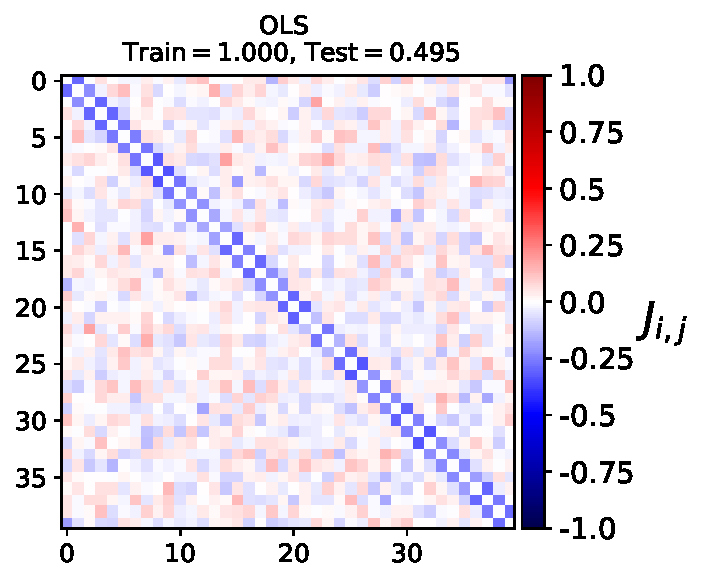
\includegraphics[scale=0.6]{latex/figures/ising_J_ols.pdf}
\end{center}
\caption{figure text}
\label{fig:j_ols}
\end{figure}

\autoref{fig:j_lmbda} shows the coupling matrices obtained by performing Ridge and Lasso regression with different regularization parameter, $\lambda$, values.

\begin{figure}[H]
\captionsetup[subfigure]{labelformat=empty}
\centering
\subfloat[]{{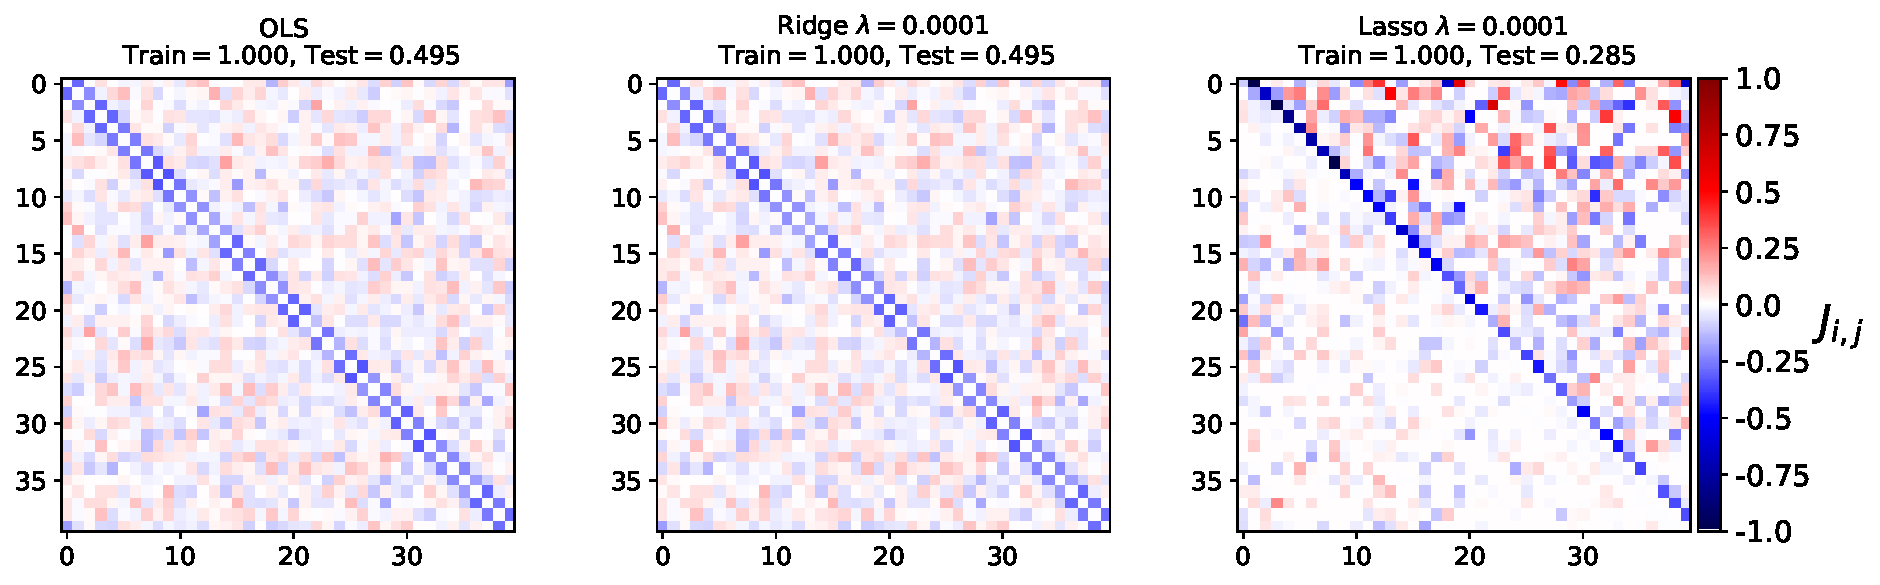
\includegraphics[scale=0.35]{latex/figures/ising_J_lmbda_0_0001.pdf}}}
\qquad
\subfloat[]{{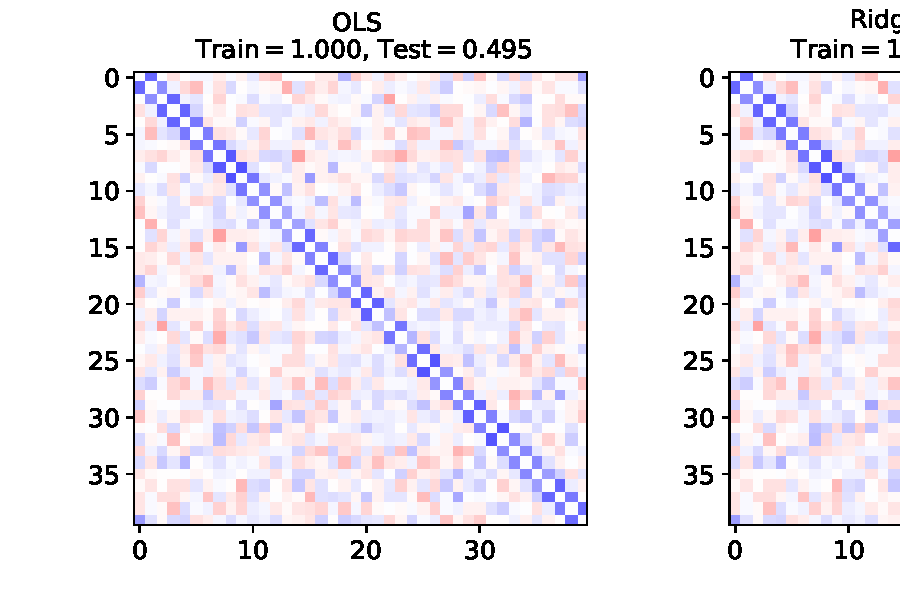
\includegraphics[scale=0.35]{latex/figures/ising_J_lmbda_0_001.pdf}}}
\qquad
\subfloat[]{{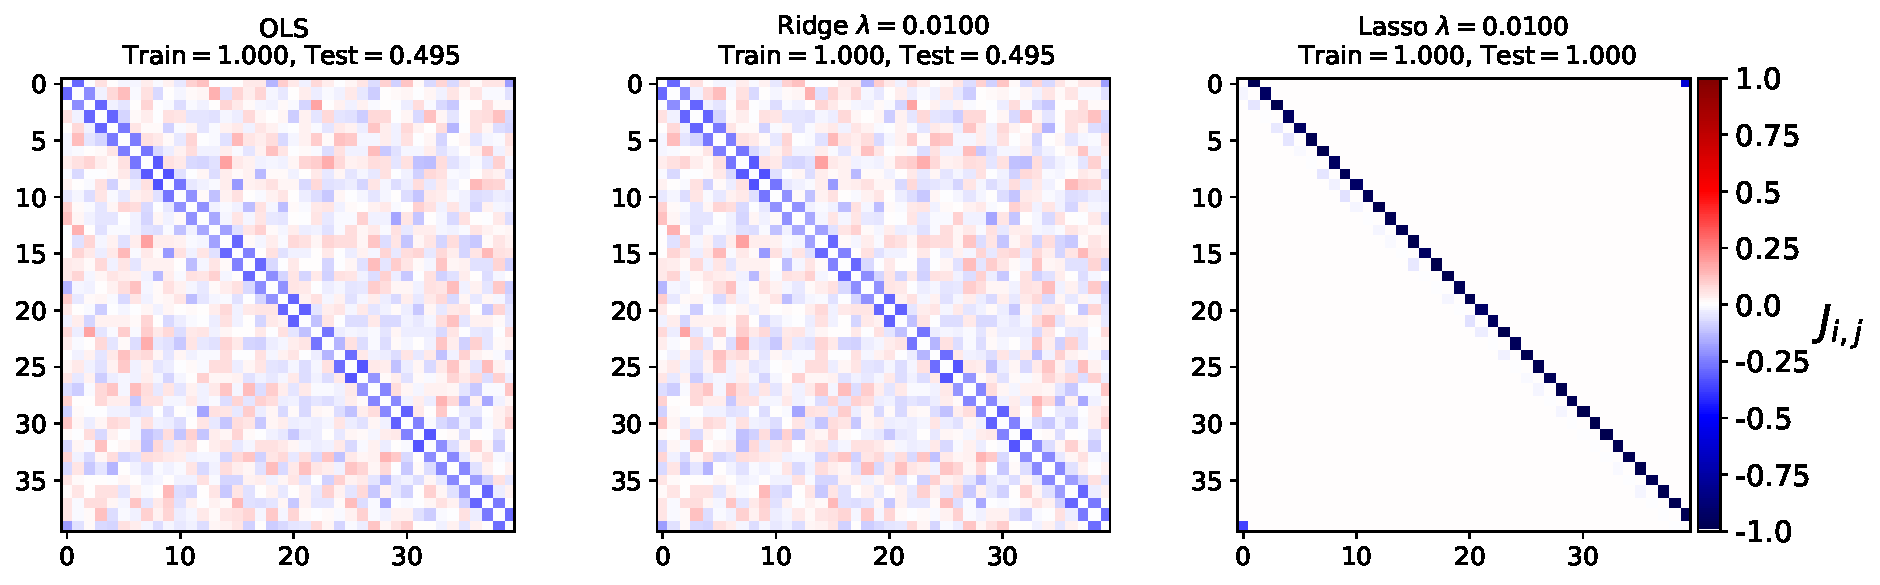
\includegraphics[scale=0.35]{latex/figures/ising_J_lmbda_0_01.pdf}}}
\qquad
\subfloat[]{{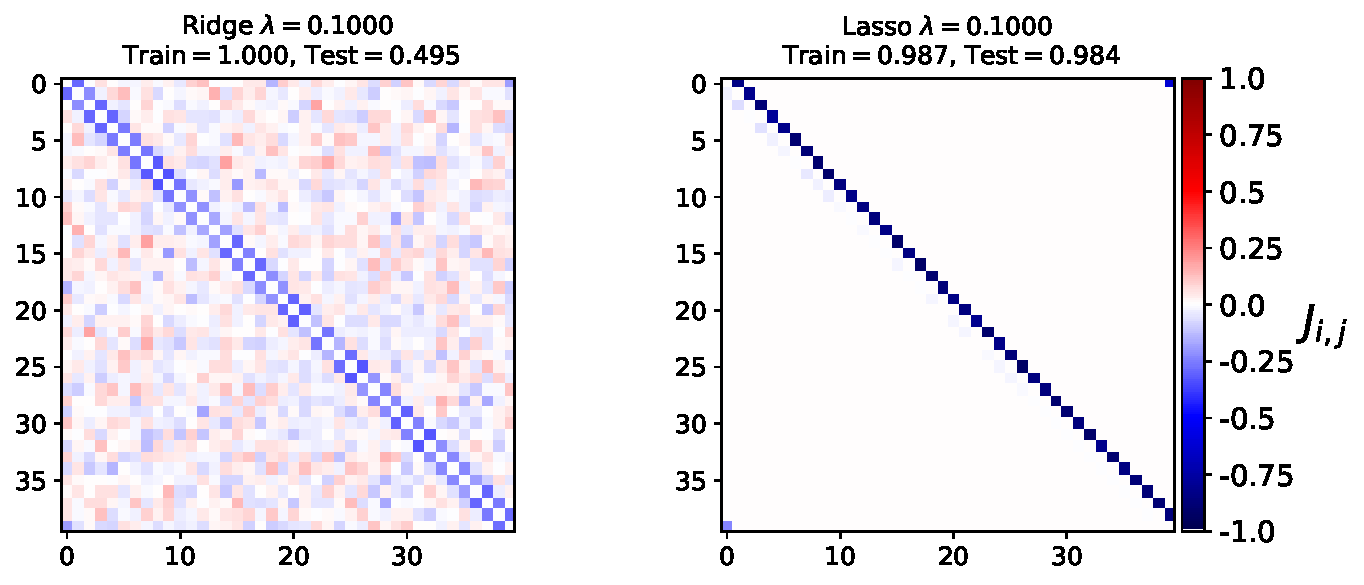
\includegraphics[scale=0.35]{latex/figures/ising_J_lmbda_0_1.pdf}}}
\qquad
\subfloat[]{{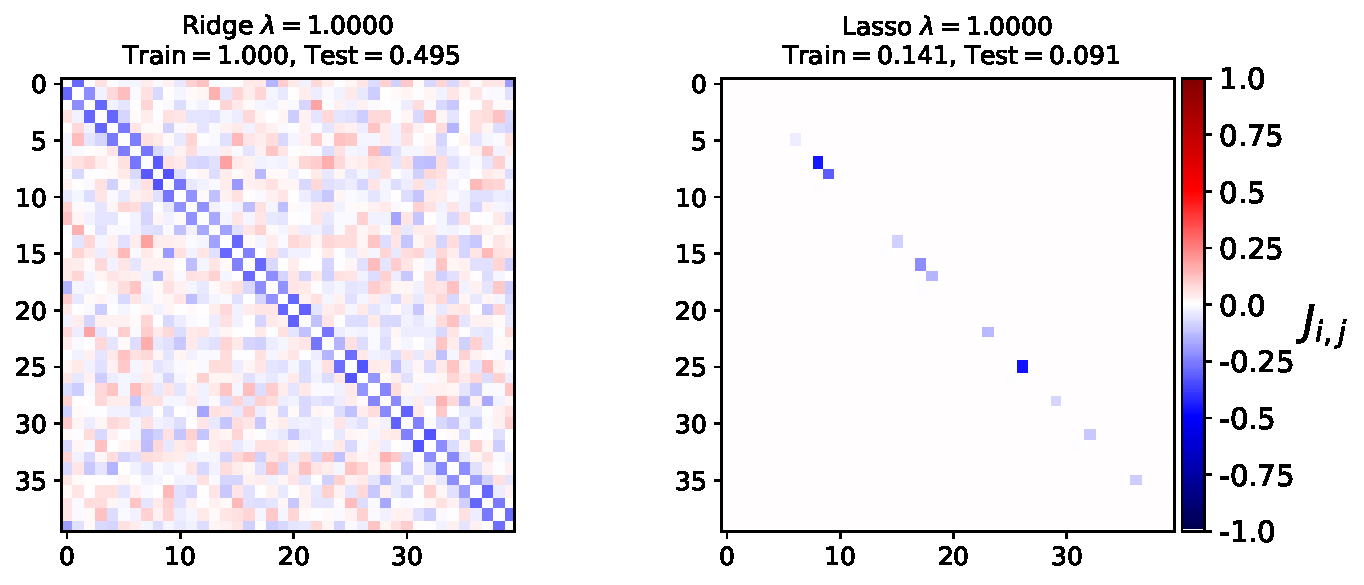
\includegraphics[scale=0.35]{latex/figures/ising_J_lmbda_1_0.pdf}}}
\qquad
\subfloat[]{{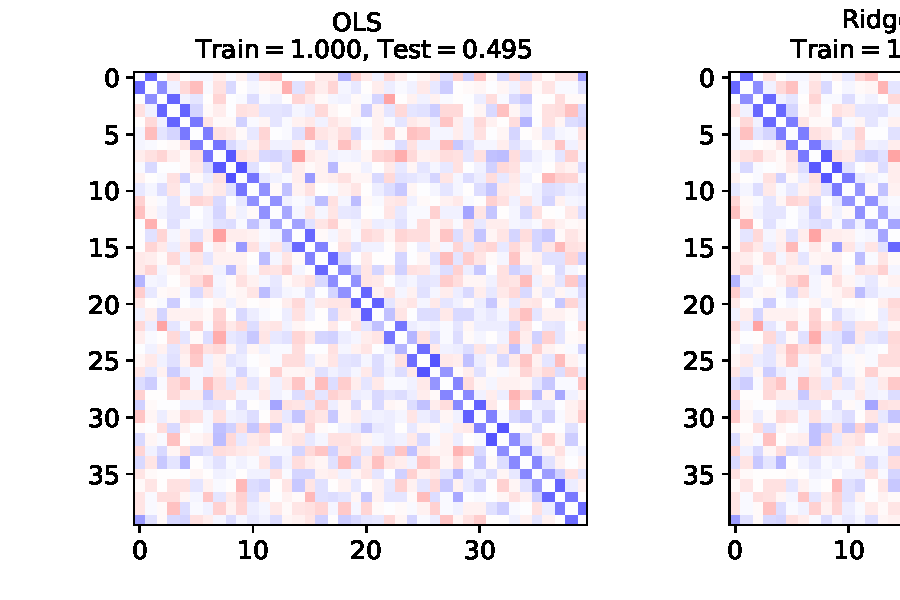
\includegraphics[scale=0.35]{latex/figures/ising_J_lmbda_10_0.pdf}}}
\qquad
\subfloat[]{{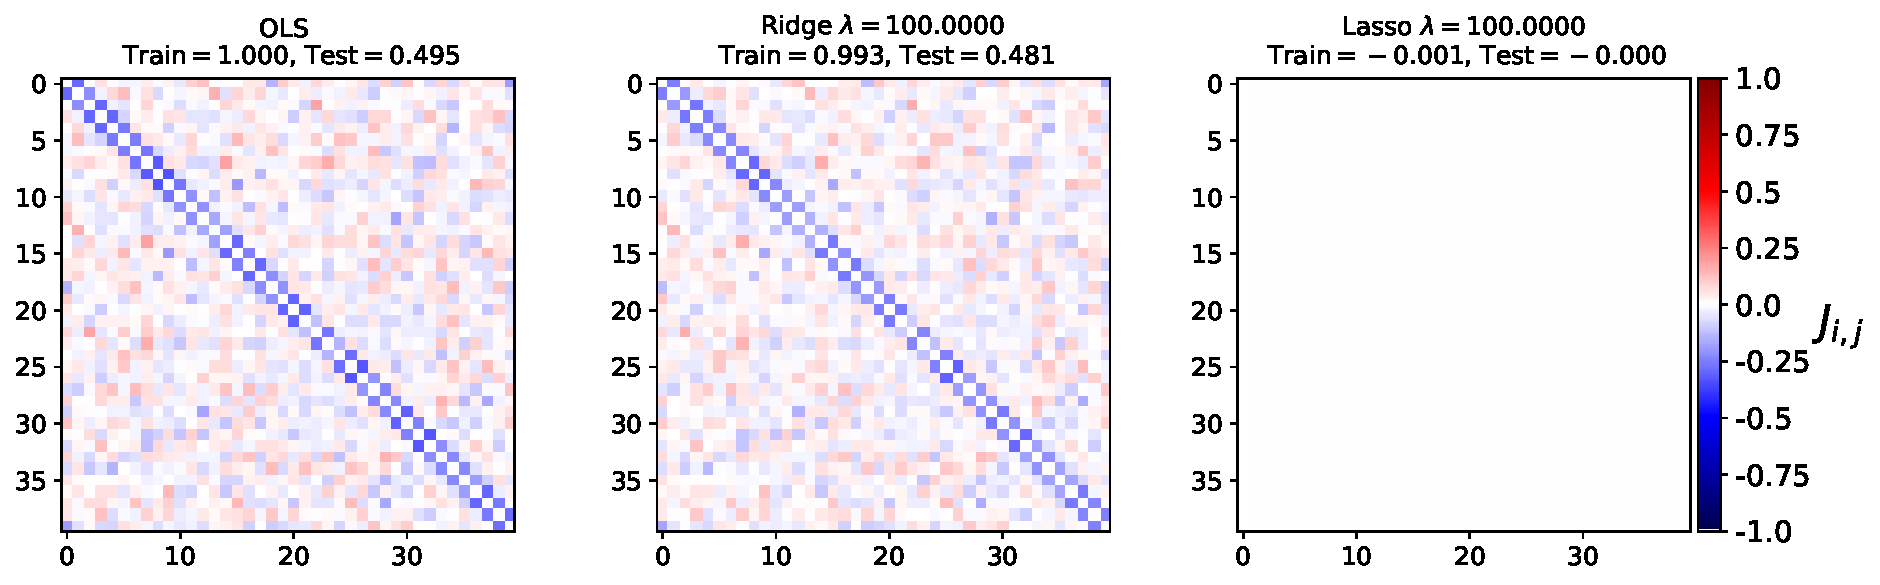
\includegraphics[scale=0.35]{latex/figures/ising_J_lmbda_100_0.pdf}}}
\qquad
\subfloat[]{{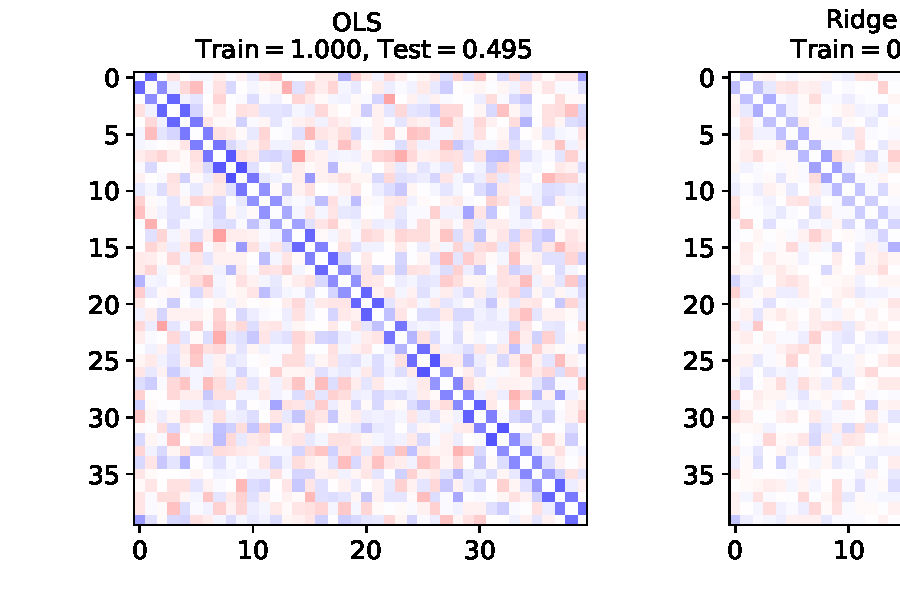
\includegraphics[scale=0.35]{latex/figures/ising_J_lmbda_1000_0.pdf}}}
\qquad
\subfloat[]{{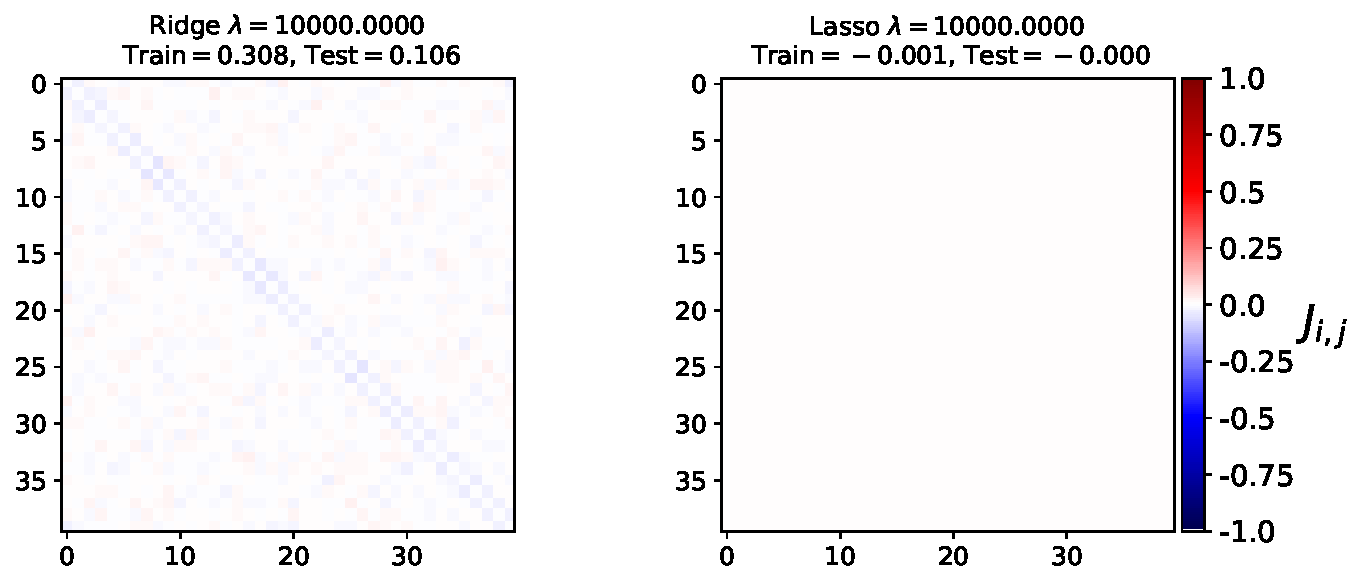
\includegraphics[scale=0.35]{latex/figures/ising_J_lmbda_10000_0.pdf}}}
\qquad
\subfloat[]{{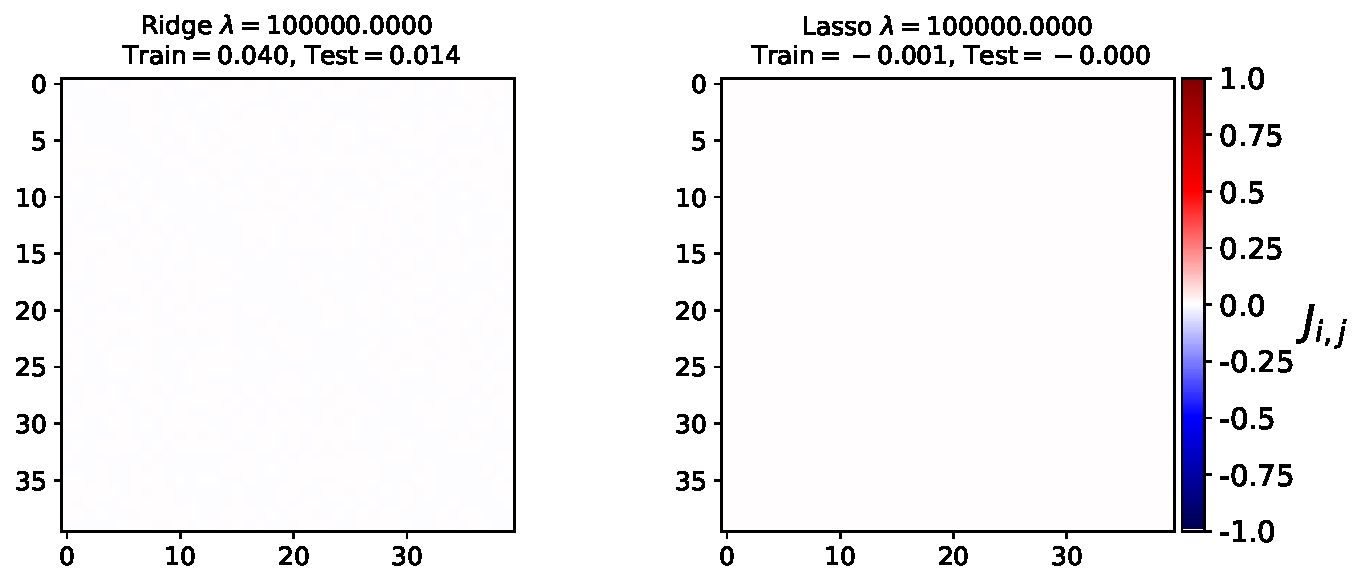
\includegraphics[scale=0.35]{latex/figures/ising_J_lmbda_100000_0.pdf}}}
\caption{figure text}
\label{fig:j_lmbda}
\end{figure}


\autoref{fig:performance_lmbda_1d} shows the $R^2$ score and MSE as a function of the regularization parameter $\lambda$.

\begin{figure}[H]
\centering
\subfloat[]{{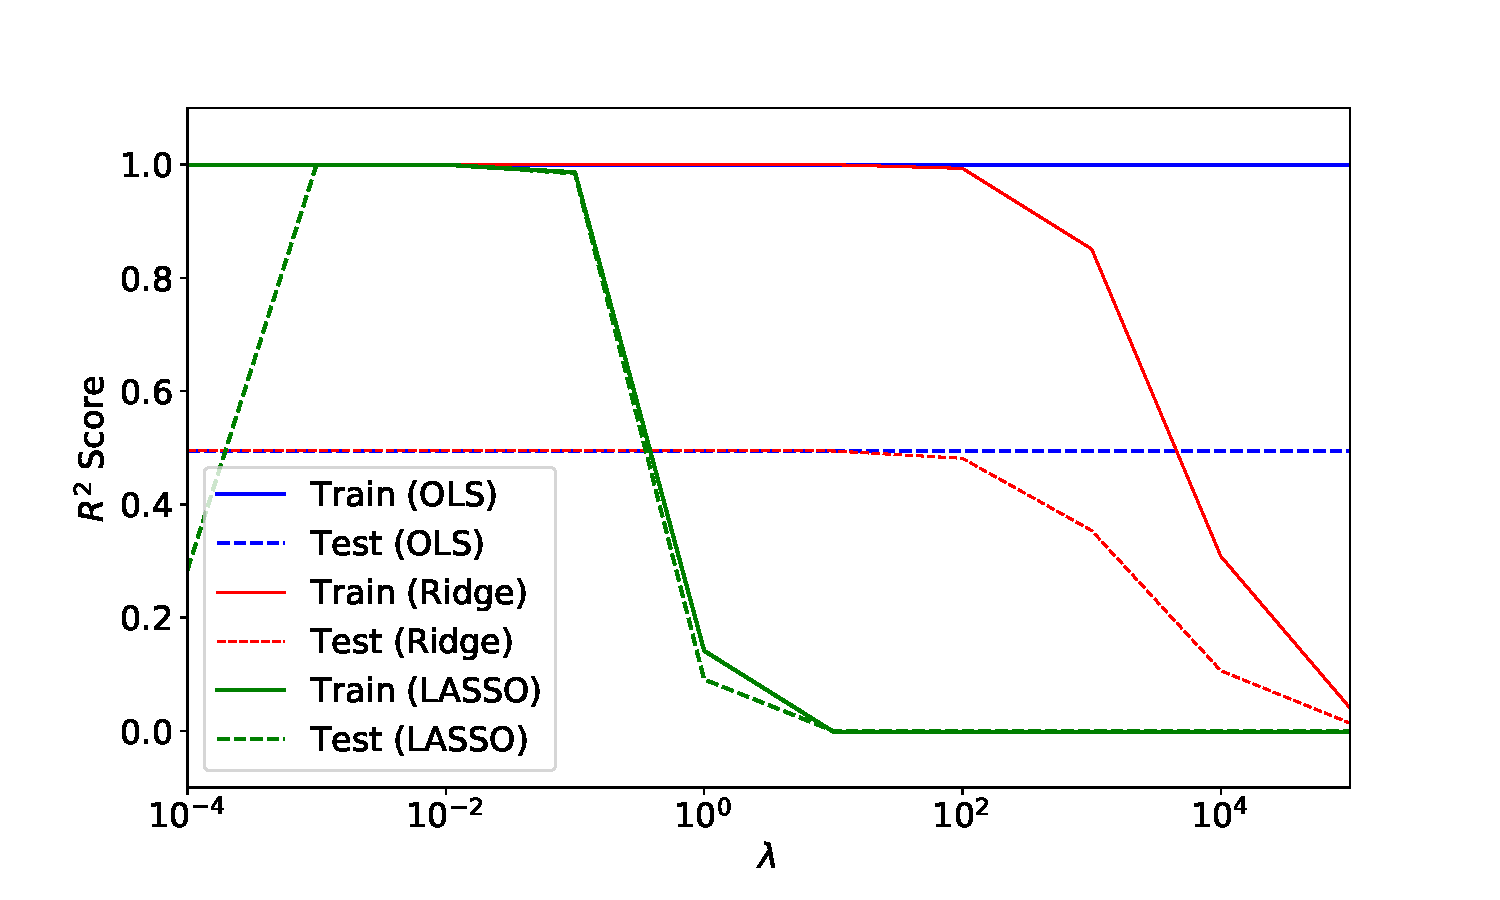
\includegraphics[scale=0.5]{latex/figures/ising1D_r2_vs_lmbda.pdf}}}
\qquad
\subfloat[]{{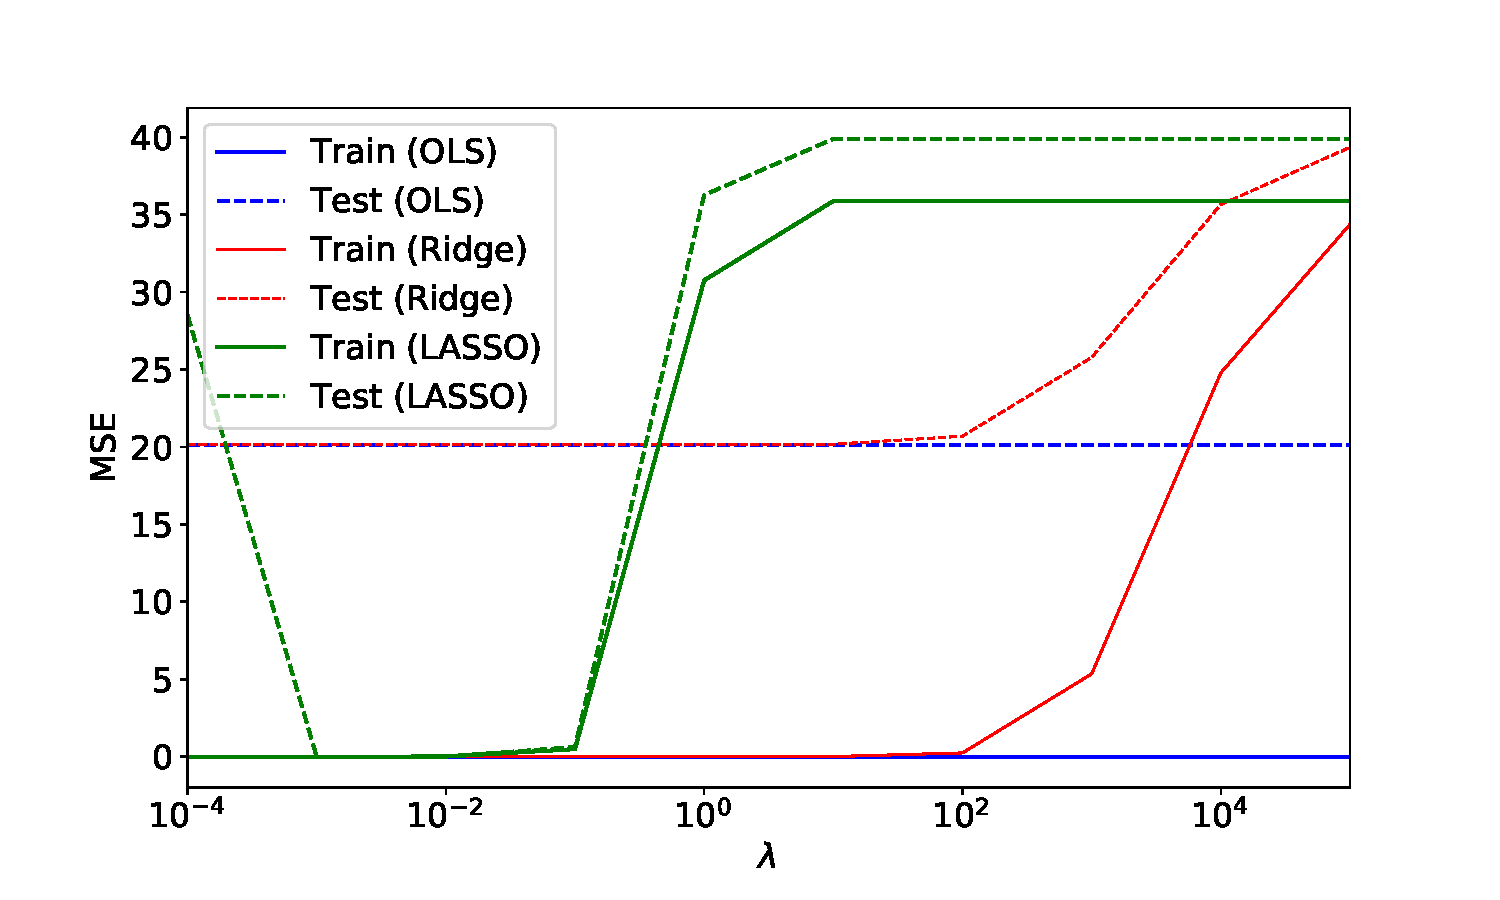
\includegraphics[scale=0.5]{latex/figures/ising1D_mse_vs_lmbda.pdf}}}
\caption{figure text}
\label{fig:performance_lmbda_1d}
\end{figure}


%----------------------------------------------------------------
\subsection{Identifying 2D Ising Model Phases with Logistic Regression}\label{sec:results logreg}
%----------------------------------------------------------------

\autoref{fig:2d_ising_states} shows some states from the data set for both the ordered and disordered phase, and the critical region as well. 

\begin{figure}[H]
\begin{center}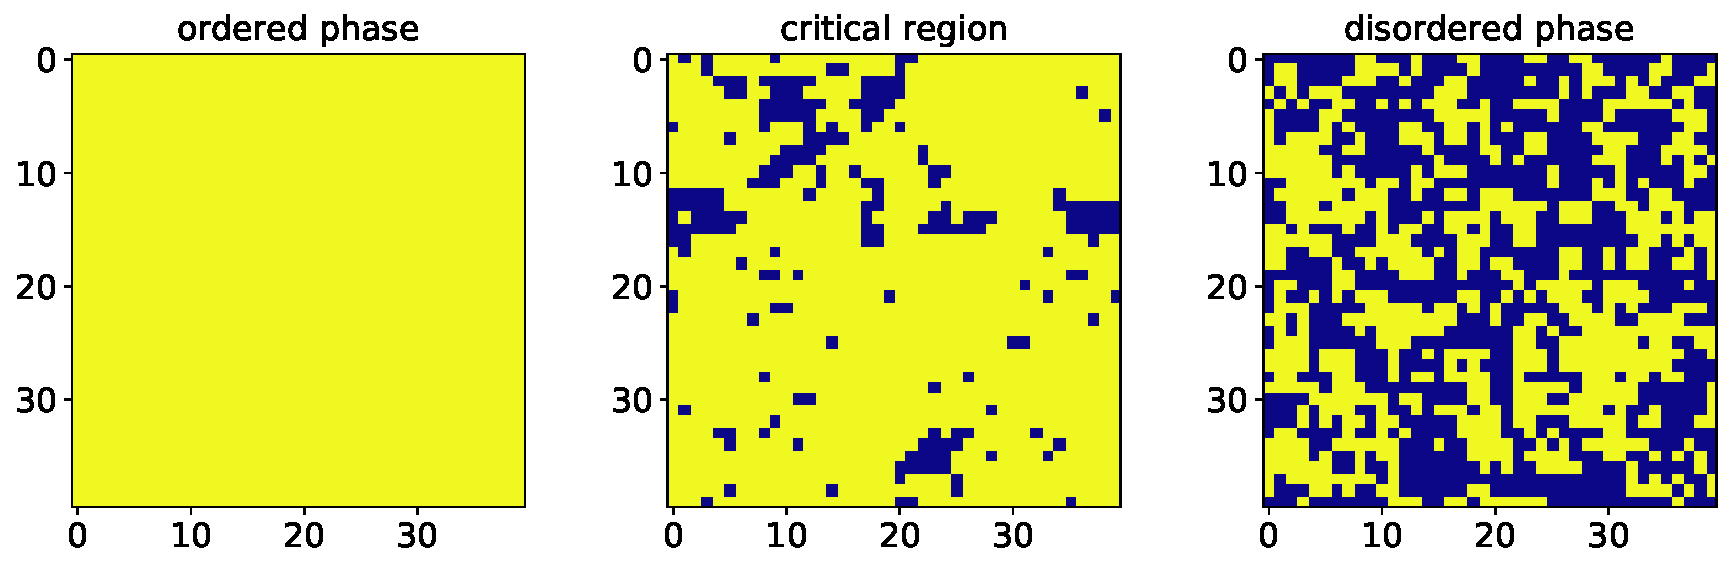
\includegraphics[scale=0.5]{latex/figures/ising_2d_states.pdf}
\end{center}
\caption{figure text}
\label{fig:2d_ising_states}
\end{figure}

%----------------------------------------------------------------
\subsection{ Regression on Energy of Generalized Ising Model using NeuralNetworks}\label{sec:results NN reg}
%----------------------------------------------------------------

\begin{figure}[H]
\centering
\subfloat[]{{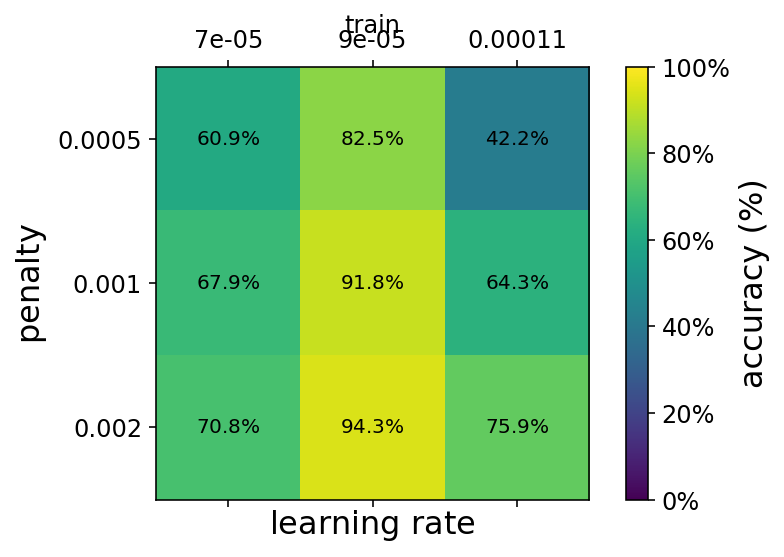
\includegraphics[scale=0.5]{latex/figures/NN_reg_train}}}
\qquad
\subfloat[]{{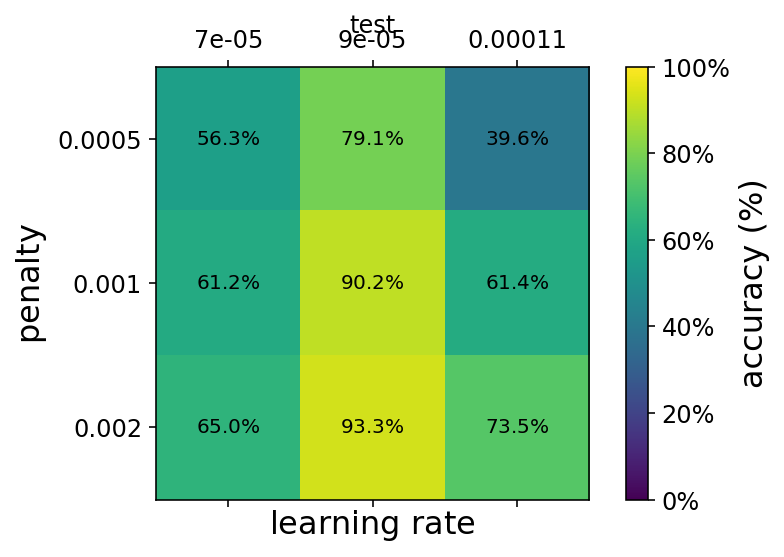
\includegraphics[scale=0.5]{latex/figures/NN_reg_test}}}
\caption{R2-score of several neural networks trained and tested on energies produced using the real Ising model \autoref{eq:ising 1D energy}, spin features produced using the generalized Ising model \autoref{eq:general}. All networks have a single hidden layer of 400 neurons, using $\tanh$ as activation, squared loss as cost function, and L2-regularization. They were trained using a grid search on learning rate and penalty}
\label{fig:NN_reg}
\end{figure}

Figure \autoref{fig:NN_reg} shows the R2-score different neural networks predicting the energy of the Ising model, using features produced by the Generalized Ising model. As the real Ising model only include local coupling, only $80$ of the $1600$ features of the generalized model actually contribute to the energy. The interesting question to explore if the network is able to pick out the useful features and ignore the others. From the figure, we see that the more heavily penalised models perform generally better. In the same manner that Ridge and Lasso help linear regression suppress features of less importance and reduce variance, the regularizing the network produces better models, presumably by suppressing the weights connecting to the redundant features. 

\begin{figure}[H]
\centering
\subfloat[]{{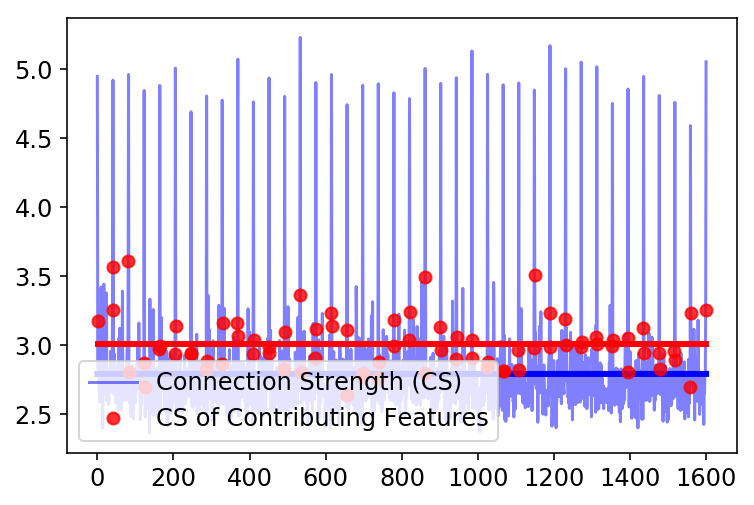
\includegraphics[scale=0.5]{latex/figures/pen1.png}}}
\qquad
\subfloat[]{{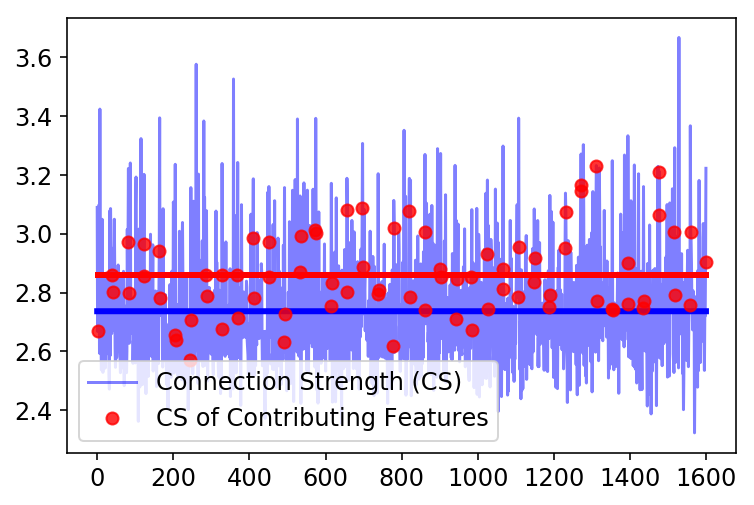
\includegraphics[scale=0.5]{latex/figures/pen2.png}}}
\qquad
\subfloat[]{{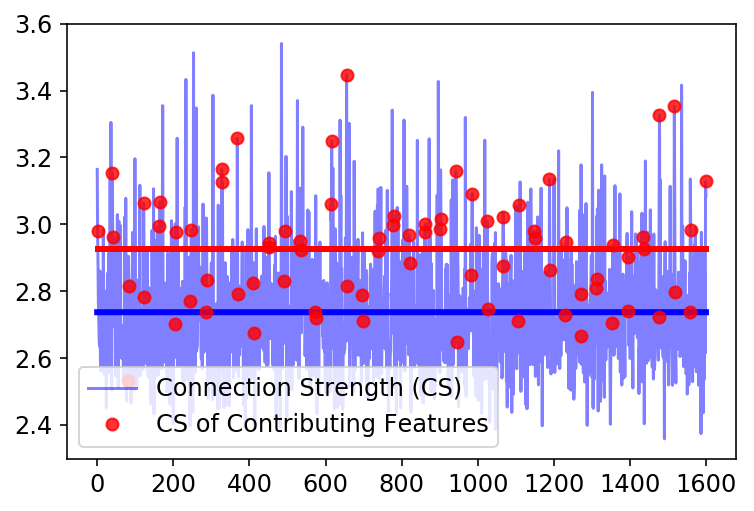
\includegraphics[scale=0.5]{latex/figures/pen3.png}}}
\caption{Connection streng}
\label{fig:NN_reg}
\end{figure}

To elaborate the previous point, figure \autoref{fig:NN_CS} visualises the Connection Strength(CS) \autoref{eq:CS} of all the inputs, with the CS of the contributing inputs highlighted by a red dot. Also the averages of the two groups are plotted. 







%----------------------------------------------------------------
\subsection{Identifying 2D Ising Model Phases with Neural Networks}\label{sec:results NN reg}
%----------------------------------------------------------------